\chapter{Introduction}
\vspace*{-2em}
In computer science, machine learning is a set of methods for learning models from examples that accurately perform tasks on new or unseen data without explicitly codifying all instructions. This automation of programming provides a time- and cost-effective alternative to otherwise manually created software solutions, making machine learning popular and widely used for many applications.

However, the relative lack of human supervision in their creation makes it hard to fully understand the inner workings of trained models and limits the ability to verify that the models work correctly. Even though it is possible to statistically verify the correctness of a model by testing it against an unseen dataset whose ground truth is known, models can unknowingly utilize latent variables that should not be used. Knowledge about those factors is often implicit in the domain of the task and neither encoded in the data nor the model. Human expertise is needed to detect and encode them explicitly or to block them out.

For example, Caruana~\etal\cite{Caruana:2015:IMH:2783258.2788613} built a Generalized Additive Model with pairwise interaction ($GA^2M$) to predict mortality risk for hospitalized patients with pneumonia, a potentially life-threatening lung infection. This area of machine learning is called predictive modeling and uses machine learning to predict a certain outcome, in this case mortality risk, based on values of several input features, in this case laboratory measurements, comorbidities, or patient demographics, and is trained from and applied to many instances. It is not feasible to individually check each prediction of the model manually. However, the machine learning algorithm $GA^2M$ used for this study is an intelligible model, that sacrifices parts of its predictive quality in favor of being understandable by humans. This enabled the authors to inspect how features contributed to the predicted outcome. One of their findings was that the model associated having asthma, a chronic lung disease, with a lower mortality rate for pneumonia patients. However, this combination of diseases is known to have a significantly \emph{increased} mortality rate. The authors double checked their data and found that this phenomenon actually occurred in their dataset and thus appeared as correct prediction in their model. After further investigation it became clear that this bias in the dataset stemmed from patients, with those conditions, being treated with intensive care thus lowering their mortality risk below the average. Outside of a hospital the risk of those patients would have been significantly higher. The model, however, only learnt about hospitalized patients which led to it being confident in this false association.

The above example illustrates the need for human understanding and supervision in machine learning and the incorrect correct result could easily be identified since the authors used a special, intelligible, model. However, not all models used in machine learning are, or even attempt to be, easily interpretable by human experts. To counteract this, visual analytics has been successfully used to visualize machine learning processes in order to understand and gain insights into predictive models. Visual analytics is the area of studying interactive graphical representations of abstract information with the help of computational and statistical procedures, in order to effectively analyze complex data. With regards to understanding the decision making of predictive machine learning models, there are two main strategies: white-box and black-box analysis \cite{class_signatures}.

% \section{White-box vs. Black-box Analysis}
In white-box analysis the main focus lies in communicating the internal structure of the model at hand. That is, the analysis is based on the assumption that knowing the full internal state of a model and being able to manually retrace decisions made by it, helps understanding the \emph{behavior} of the model in general.

In this work we will focus on black-box analysis whose focus is on communicating external behavior of a model. That is, no information about the model itself is utilized during the analysis but rather typically inferred from observing how the model reacts to carefully crafted inputs. Compared to white-box analysis there are several advantages.

As white-box analysis relies on the internal structure and thus the nature of a particular model type, such as the $GA^2M$ mentioned above, a method developed for one type might not be applicable to a different type. This limits the usefulness of white-box analysis as every new algorithm demands often an entirely new form of representation. Since black-box analysis is model independent findings are universally applicable.

\newcommand\Tstrut{\rule{0pt}{2.5ex}}
\begin{table}
     \begin{tabular}{cl|cl} 
     & \textbf{White-box} & & \textbf{Black-box} \\
     \hline
     \hline
    $\oplus$ & Deep understanding of decisions & $\ominus$ & External behavior only \Tstrut \\
    $\oplus$ & Always reflects the true & $\ominus$ & Not guaranteed to reflect model \Tstrut \\
    & decision making process & & decisions truthfully in all cases \\
    $\oplus$ & Full internal state available & $\ominus$ & Limited knowledge of \Tstrut \\
    & & & model specifics \\
    \hline
    $\ominus$ & Model specific techniques & $\oplus$ & Reusable techniques \Tstrut \\
    $\ominus$ & Complexity / interpretability & $\oplus$ & Complexity / interpretability \Tstrut \\ 
    & data and model dependent & & independent of data and model \\
    $\ominus$ & Switching to interpretable model & $\oplus$ & No performance considerations \Tstrut \\
    & incurs performance penalty & & necessary \\
    \end{tabular}
    \centering
    \vspace*{-0.5em}
    \caption{Comparison of black-box and white-box explanation strategies. $\oplus$ indicates advantages of a technique while $\ominus$ indicates drawbacks.}
    \vspace*{-0.75em}
    \label{tab:blackvswhite}
\end{table}

Another drawback of white-box analysis is its scalability to the complexity of the model. Many solutions do not sufficiently scale as models become more complex. For example, a decision tree with 5 nodes, often used as example when explaining the technique, can easily be visualized and understood in a node-link representation. This representation fails to help understanding a decision tree with hundreds or thousands of nodes. For black-box analysis the internal complexity of a model is irrelevant.

On the other hand black-box analysis also has drawbacks. Especially the limited knowledge of the underlying model allows only for an approximate understanding of its behavior as testing the entire input space would be intractable.

The main goal of this thesis is to explore how model agnostic feature contribution methods can help to gain a holistic understanding of, as well as, insights about predictive models using visual analytics. In three stages, we will show the progression from initial observations, that led us to utilizing black-box analysis, to the eventual use of aggregated instance-level explanations to understand, trust, and verify predictive models. Additionally, we show that our developed visual analytics techniques can be helpful for feature engineering.

Feature engineering is the task of deciding which features will be collected for a particular machine learning problem and how those features are pre-processed or transformed in order to create favorable model results. It requires both expertise of the problem domain, as well as, experience in picking and manipulating features in ``the right way". For the most part, feature engineering cannot be automated and is typically seen as ``black-art" as it relies on intuition and creativity of the modeler \cite{Domingos:2012:FUT:2347736.2347755}.

% \section{\infuse}
In the first stage we analyze and compare different feature selection strategies. Feature selection is a pre-processing step that, unlike feature engineering, algorithmically determines the possible predictive impact of a feature. Only the most impactful features are then used as input for the predictive modeling process. This is often necessary as a larger number of features require significantly more training examples to accurately represent the valid input space without losing predictive qualities. As feature selection algorithms use similar statistical tools as many predictive modeling techniques it seems plausible to infer the importance of features in the context of decision making through feature selection in a model agnostic way.

Being able to visually compare different feature selection strategies the machine learning experts noticed that, depending on the chosen feature selection algorithm, different, mostly distinctive, feature sets were deemed to be important while, at the same time, having no significant impact on predictive performance. Additionally, from the view of a domain expert those feature sets were equally reasonable in the context of the prediction task.
This demonstrates that \textbf{inspecting} and \textbf{comparing alternate settings} lets machine learning experts develop insights that \textbf{overwrite} their \textbf{initial intuitions}.
Also, concluding that rankings from feature selection algorithms are not informative enough to provide the importance of features in the context of understanding model decisions, a more powerful model agnostic approach is needed.

% \section{\prospector}
In the second stage we explore the influence of features in the decision making process of predictive models through a technique called partial dependence. Partial dependence computes feature impact on model outcomes by systematically probing the model with artificial inputs. That is, while keeping the rest of the input values the same, the inspected feature assumes all possible values showing the relationship of feature values to the prediction score. Aggregated over all observed instances, the general behavior of the model with respect to a given feature can be inferred. By computing a novel feature importance score from partial dependence relationships unusual and interesting relations can be found quickly without having to inspect all, often several thousand, features.

Analyzing partial dependency relationships on diabetes prediction models trained on electronic medical records containing patient demographics, diagnoses, medications, and laboratory results, using our method we gained several insights. Firstly, we showed that logistic regression models are not expressive enough to accurately model the complex relationships of certain features to the outcome. Secondly, imputation of missing values, using the population average in laboratory results, caused the model to become uncertain close to the normal value range of laboratory tests. Lastly, we found that the model used a proxy variable indicating the number of doctor visits as predictor of the healthiness of a patient. However, this is \emph{not} a valid predictor. Even though a patient is likely to visit a doctor more often if she is sick, the reverse cannot be said. The above findings show how \textbf{partial dependence} with the proposed \textbf{feature importance score} allow analysts to effectively \textbf{detect model errors} related to \textbf{over-} and \textbf{under-fitting}, \textbf{imputation}, and \textbf{incorrect cause-effect relationships}.
However, a major drawback of using partial dependency is its limitations on extending it to relations of multiple features to the predicted outcome.

\begin{figure}[t]
\centering
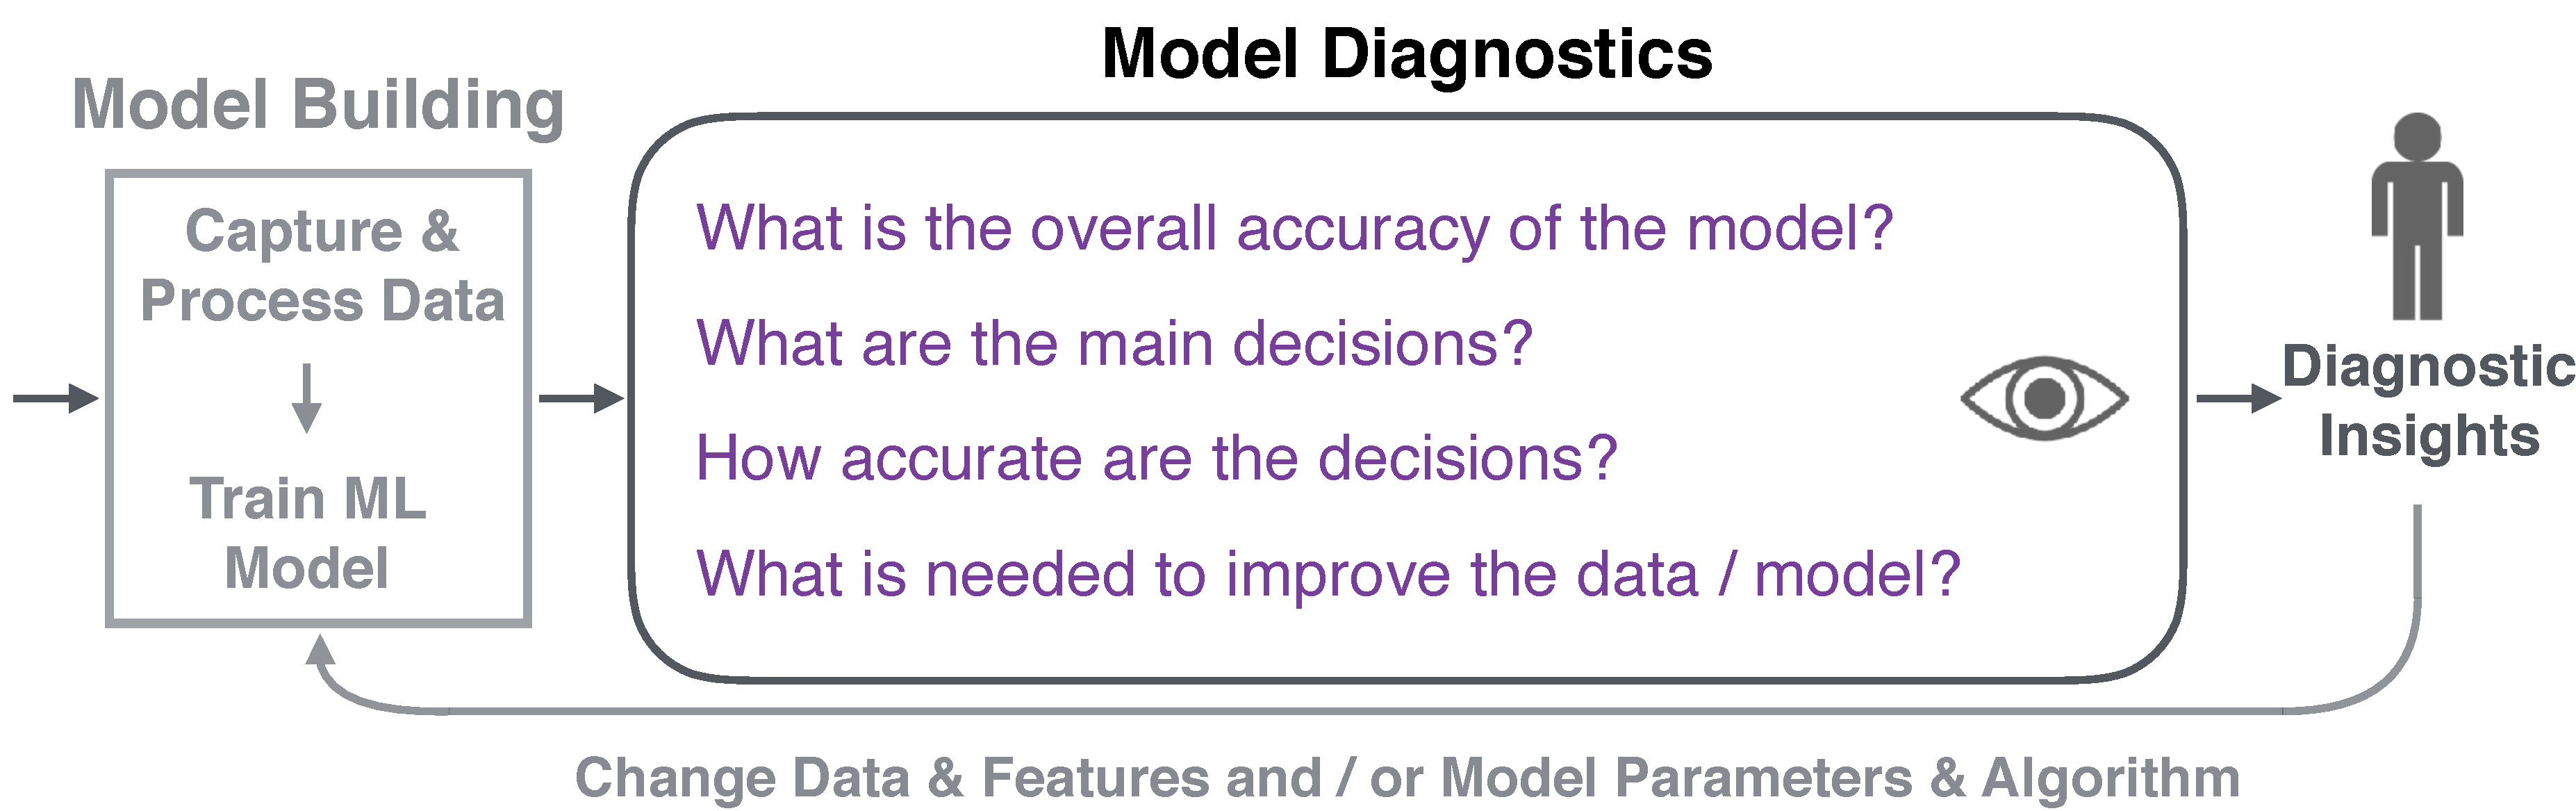
\includegraphics[width=\textwidth]{figs/workflow_large}
\caption[The model diagnostic workflow.]{
The proposed \textit{model diagnostic} workflow extends the conventional \textit{model building} workflow in machine learning for enabling domain experts to reason about the semantic validity of the decisions made by any model through multiple linked visualizations.
This ultimately helps to improve data acquisition and model generation processes belonging to the original workflow.
}
\label{figs:workflow_intro}
\end{figure}

% \section{Model Diagnostic Workflow}
In the third stage, we overcome this limitation by leveraging instance-level explanations. Instance-level explanations are defined as the smallest change, to an instance vector, necessary to change the predicted outcome label. Aggregating over those explanations and statistically analyzing the resulting instance subsets, proves as powerful novel approach for understanding the behavior of a model. Additionally, we propose a model diagnostic workflow (see \figref{figs:workflow_intro}) that helps identify flaws in the \emph{input data}, used to train and test the model.

We use this workflow to analyze a predictive modeling problem revolving patient admission to a hospital, of patients in the emergency department of said hospital. Accurately predicting whether a patient eventually gets admitted to the hospital helps reducing costs. The major limiting factor of this prediction task is the need for input features readily, and electronically, available at the earliest point possible. To this extend we initially used features of prescribed medications as this information is immediately available electronically. Our analysis showed that there are clear groups of patients where the predictive model is very helpful. However, there are some groups of patients where it is impossible for the predictive model to make accurate predictions given the provided information. One of those groups is patients receiving Diatrizoate Meglumine, a contrast medium for CAT or PET scans. This medication only indicates that a scan was performed, but does not carry information about the result of the scan. However, the result of the scan is the deciding factor whether a patient needs further care or can get sent home. Thus, with the given information it is impossible for the predictive model to make a decision that performs better than random guessing. Including more information in the form of additional features does indeed help with this problem but pushes the time when a decision can be made further back. One possible solution is to utilize the predictive model only for the confident groups of patients and wait for the doctors' decisions in other cases. This example illustrates that it is not only possible to \textbf{understand decision making} of a predictive model through the \textbf{model diagnostic workflow} based on \textbf{aggregated instance level explanations}, but also how it can be applied for \textbf{semantic validation} and \textbf{feature engineering} on the input data.

\begin{table}[t]
     \begin{tabular}{l|c|c|c} 
     \textbf{Approach} & \makebox[0pt][l]{\textbf{Instances}}\phantom{Aggregated} & \textbf{Aggregated} & \makebox[0pt][l]{\textbf{Global}}\phantom{Aggregated} \\ 
     \hline
     \hline
     \infuse & & & X \Tstrut\\
     \hline
     \prospector & X & & X \Tstrut\\
     \hline
     \textit{Model diagnostic workflow} & & X & \Tstrut\\
    \end{tabular}
    \centering
    \vspace*{-0.5em}
    \caption{Locality of decision analyses of the presented approaches. \textbf{Instances} refers to analyzing decisions for one instance at a time. \textbf{Aggregated} refers to analyzing decisions for groups of instances and \textbf{Global} refers to analyzing decisions globally without inspecting decisions for individual instances.}
    \vspace*{-0.75em}
    \label{tab:locality}
\end{table}

\todo{fill in latest work}
In addition to those promising results, there is still work to do.
It still needs to be shown that the proposed workflow of statistical analysis of instance-level explanations can be successfully applied to other data types than binary feature vectors, such as numerical features or highly redundant features such as found in images.
Early results in this direction indicate that it might be beneficial to abandon the focus on features to explain machine learning models, but rather focus on instances directly.
That is using instance-level explanations to obtain groups of \emph{instances} with similar behavior and then visualize those groups (\eg, using techniques proposed by \cite{seekaview}) in order to \emph{implicitly} explain them.
This provides more flexible explanations than those proposed earlier as their capability goes beyond ``Feature A and feature B positively impact the prediction for this group of instances" to also allow insights of the form ``The number of circles formed by black pixels contribute positively to the prediction" which would be very difficult to formulate by a machine but are easily formulated by humans using visualizations.
Furthermore, we are going to run a study on the implications on confidence in and trust of machine learning models when using different explanation approaches.

The following document first describes the already completed stages: \infuse (\chapref{chap:infuse}), \prospector (\chapref{chap:prospector}), and the model diagnostic workflow using instance-level explanations (\chapref{chap:explainer}).
After that the progress on the current stage is described in \chapref{chap:current} and an outline for the thesis is given in \chapref{chap:thesis}.
%%%
%  Furthermore, a formalization or taxonomy of common machine learning modeling \emph{errors} in both the modeling and feature engineering steps is needed to fully determine the limitations of the proposed black-box analysis methodologies. This can be achieved by taking a survey with both machine learning and domain experts to get an understanding and relevance of different kinds of those errors.
%%%

% Machine learning is a powerful tool that is used more and more in everyday life.
% By relating independent features and targets by detecting complex associations machine learning
% helps human decision making and, in some cases, even replaces it.
% Predictive modeling using classification techniques is a very common application of machine learning.
% In this work we will primarily focus on classification but the techniques discussed can, to some extent, be
% applied in other areas of machine learning as well.

% \begin{figure}
\centering
\vphantom{7cm}
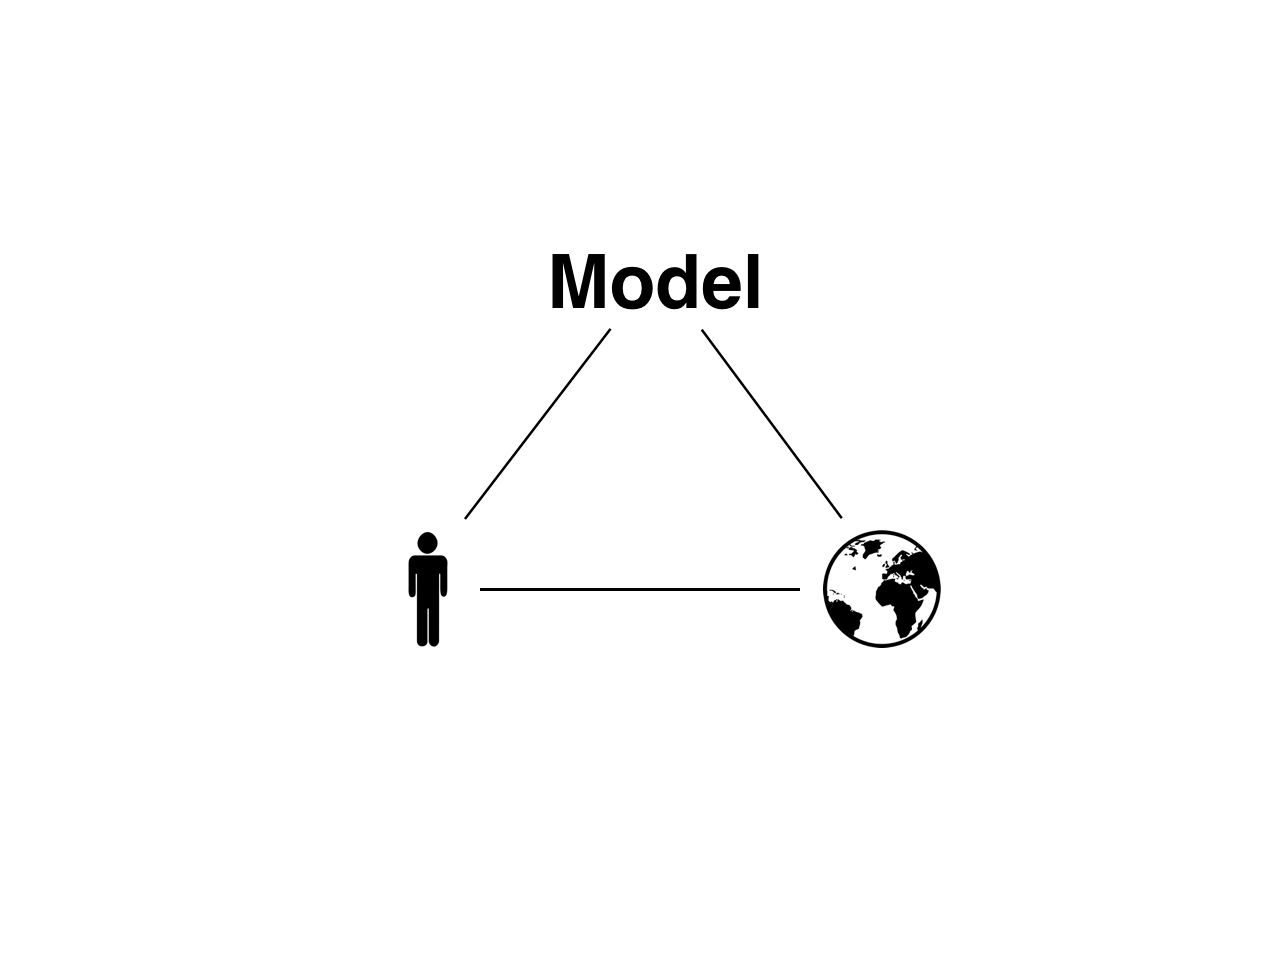
\includegraphics[trim={7cm 8cm 7cm 8cm},clip=true,width=0.275\linewidth]{figs/motivation/hmr}
~
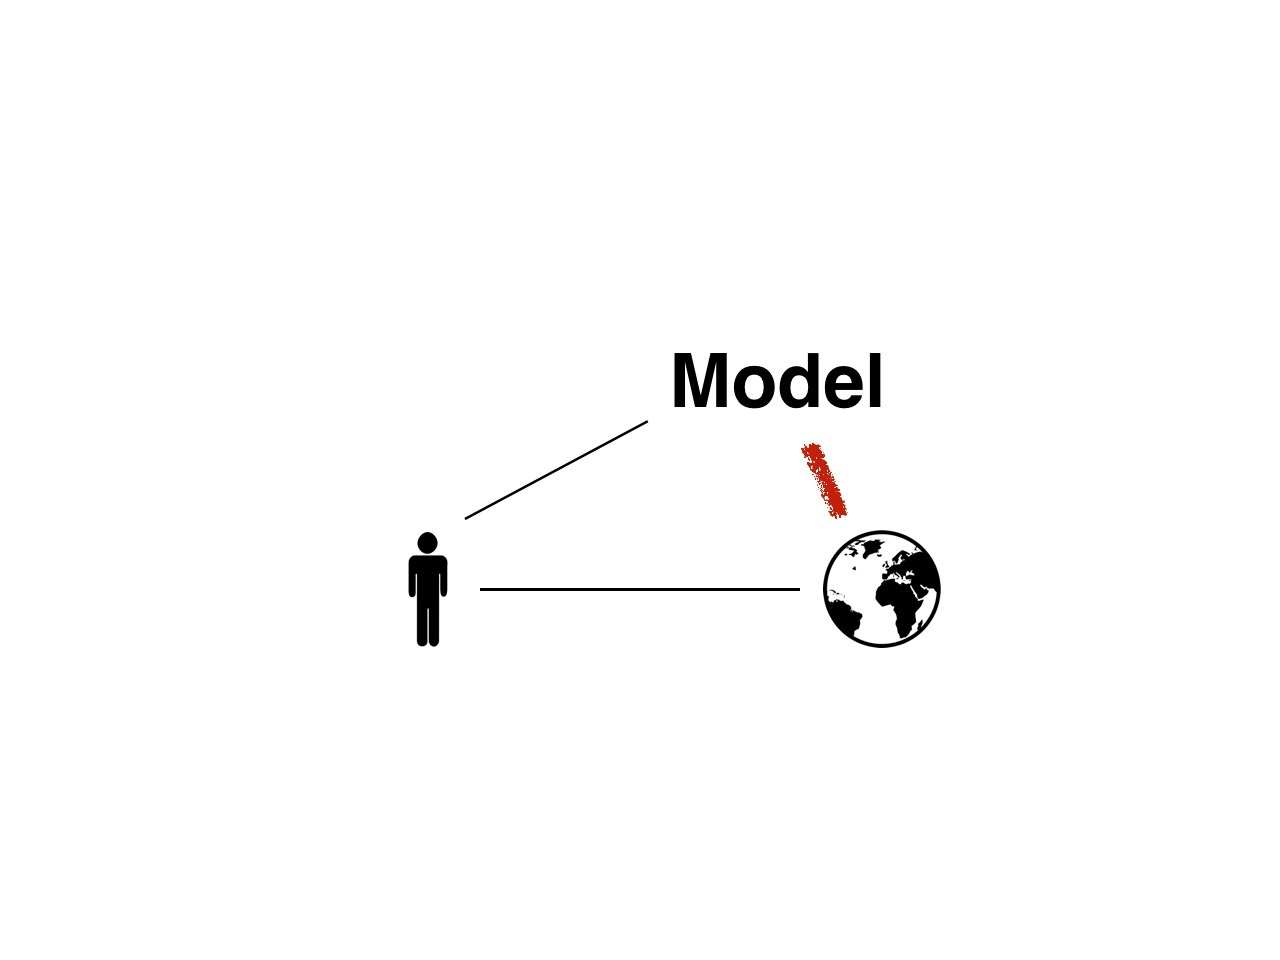
\includegraphics[trim={7cm 8cm 7cm 8cm},clip=true,width=0.275\linewidth]{figs/motivation/hmr_complex}
~
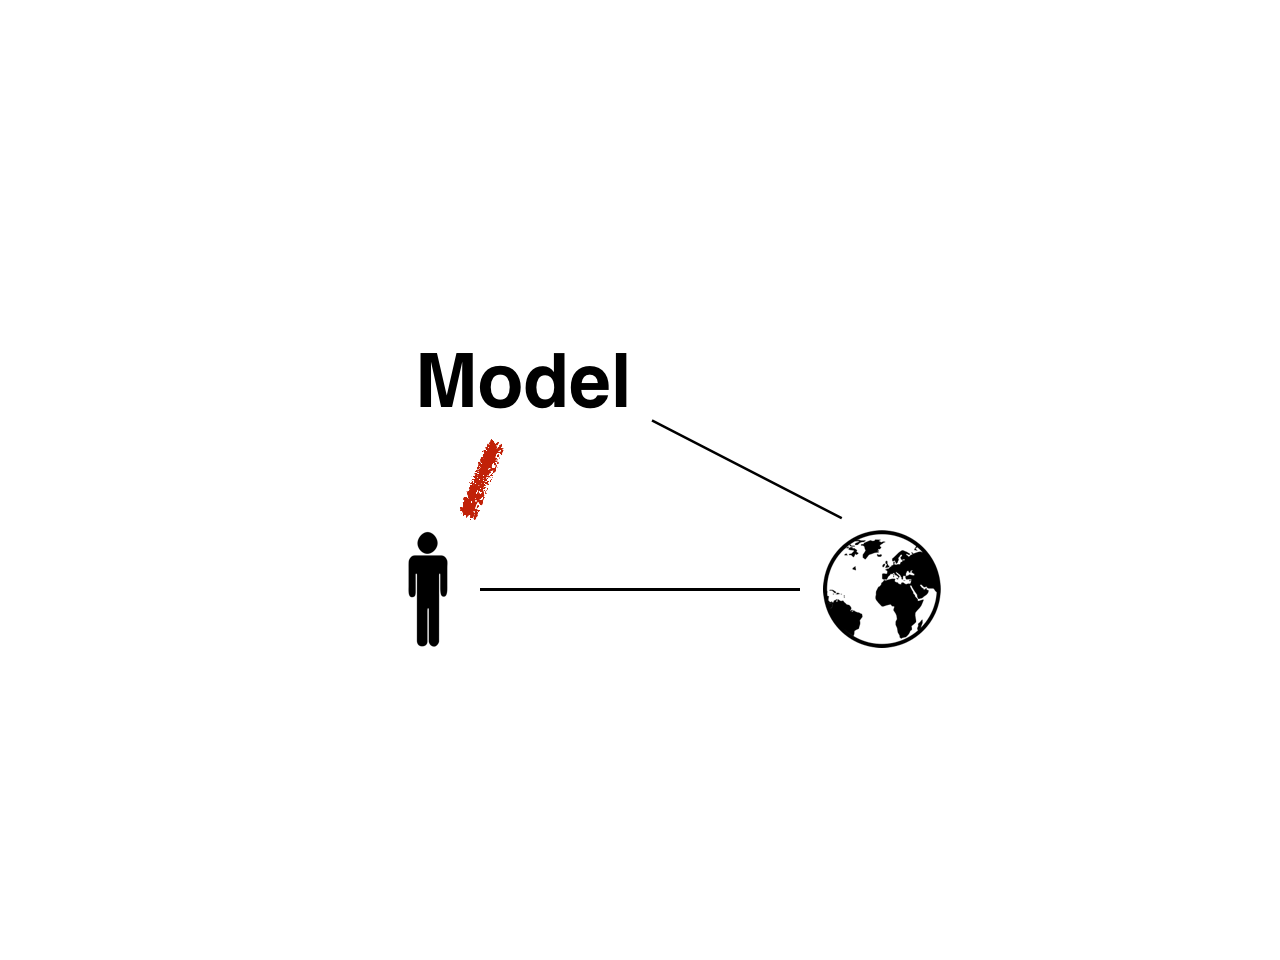
\includegraphics[trim={7cm 8cm 7cm 8cm},clip=true,width=0.275\linewidth]{figs/motivation/hmr_interpretable}
\caption{
Humans (lower left) build machine learning models (top) to understand and
predict reality (lower right). The second image illustrates how improving
machine learning models (ie., closing the gap between the model and reality)
makes it harder for humans to understand it. Likewise, simplifying the model
(ie., closing the gap between the model and the human) makes the model less
accurate (third image).
}
\label{figs:motivation_hmr}
\end{figure}

% As the scope and usage of machine predictions increases with bigger and more complex data
% the used algorithms need to also become more complex.
% However, as complexity increases it becomes harder for humans to follow the machine's decision making
% as illustrated in \figref{figs:motivation_hmr}.
% This problem of model transparency and interpretation is important and very well recognized in machine learning,
% as models with high predictive performance generally have low transparency and vice-versa~\cite{breiman2001}.

% \begin{figure}
\centering

\includegraphics[height=10.5em]{figs/motivation/ml_orig}
\raisebox{4.75em}{$\Rightarrow$}
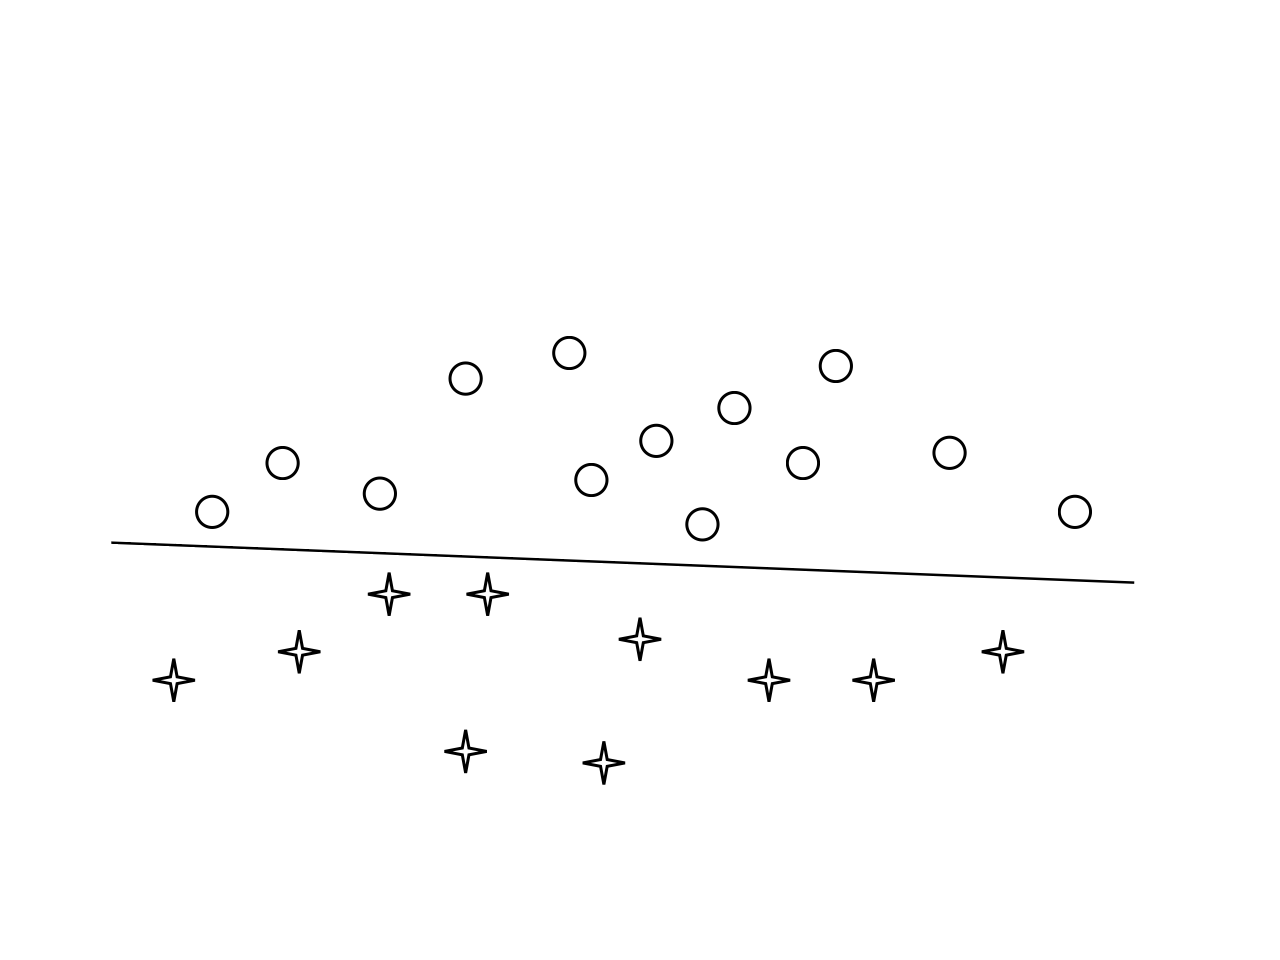
\includegraphics[height=10.5em]{figs/motivation/ml_proj}
\caption{
Machine learning algorithms transform the complex raw input space (left)
into a cleaner transformed space (right) that can be easily separated.
Transformations are often strongly non-linear, non-affine, and/or non-continuous
and thus not easy to follow or understand.
}
\label{figs:motivation_ml}
\end{figure}

% Many applications of machine learning need to be interpretable to humans even though
% sacrificing prediction performance is not desirable.
% For example, in the health care domain disease prediction using patient histories needs to be fully
% transparent and comprehensible to practitioners as lives are at stake when applying models in the real world.
% Even if a model performs well on the test data it could draw its conclusions from hidden signals or biases
% in the training data. We found many of such examples in the work presented here.

% One way of overcoming the problem of interpretability vs. performance in machine learning is to
% break down the complex models into smaller parts that are easier to understand (see \figref{figs:motivation_ml}).
% While this reduces the complexity it also reduces the generalizability of the explanations created this way.
% In the following we will explore when explanations are useful and how they can be used.

% \section{Explanations}
% Explanations for machine learning can be desirable for multiple reasons:

% \begin{description}
%     \item[Liability]
%         Decisions made by the machine have real world consequences with attached liabilities.
%         Explanations are needed to create confidence that the model avoids costly misjudgements of critical inputs.
%     \item[Trust]
%         Stakeholders need to be able to trust decisions from the model.
%     \item[Debugging]
%         Help understanding why a model behaves different than expected.
%     \item[Comparison]
%         Provide a model agnostic way of comparing different models.
%     \item[Hidden Associations]
%         Find hidden associations in the original data.
%     \item[Ambiguity Reduction]
%         By creating generalizing models and explaining their behavior a noise-free view of the data can be created.
% \end{description}

% Those explanation tasks can be performed at different steps in the machine learning process.
% In this context predictive modeling typically consists of three steps (see \figref{figs:motivation_flow}).
% First, the input data has to be prepared.
% This entails choosing which data points are eligible for modeling to ensure that no inherent biases influence
% the validity of the created model.
% Furthermore, data usually needs to be converted into features that can be used by machine learning models.
% Second, the model has to be trained on the transformed data.
% Depending on the type of the model or strategy this step includes splitting the data into cross-validation sets,
% algorithmic feature selection, and actually training the model.
% Third, the actual prediction can be performed which often entails converting class probabilities into
% concrete labels upon which decisions can be performed.

% Explanations can be separated into different categories that utilize and describe
% different stages of the predictive modeling pipeline.
% Thus, explanations can be divided into input-, output-, interaction-,
% and structure-explanations.
% Input explanations mostly work with the raw input data and can help the pre-processing.
% Output explanations analyze outputs from the machine learning model such as feature ranks
% or prediction scores.
% Interaction explanations change model inputs to observe how the corresponding model output
% changes.
% Structure explanations describe the inner values and weights of a model so decisions
% can be followed manually.

% \begin{figure}[b!]
\centering
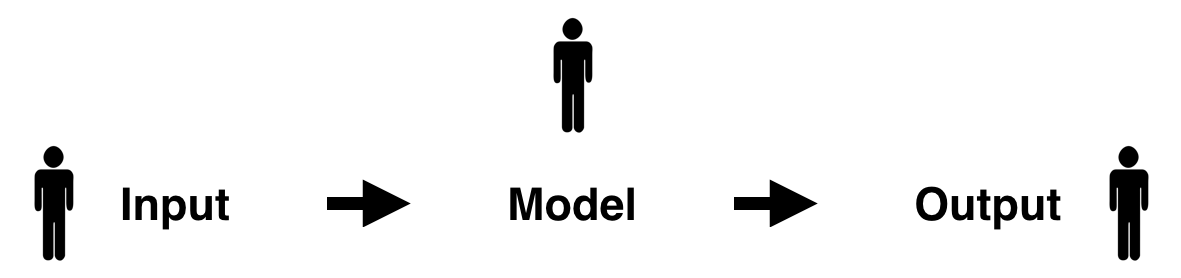
\includegraphics[width=0.7\linewidth]{figs/motivation/flow}
\caption{
The predictive modeling pipeline.
Humans symbolize where explanations are helpful.
Explanations of the model can either focus on input-output interactions
or the structure of the model.
}
\label{figs:motivation_flow}
\end{figure}

% Output and interaction explanations can also utilize model induction, which is building
% a less complex model on top of the original model's output or on a strategically chosen
% subset of data points.
% This less complex model can then be structurally described which is beneficial when
% dealing with very complex models whose structural explanations are too difficult to
% understand.

% \begin{figure}
\centering
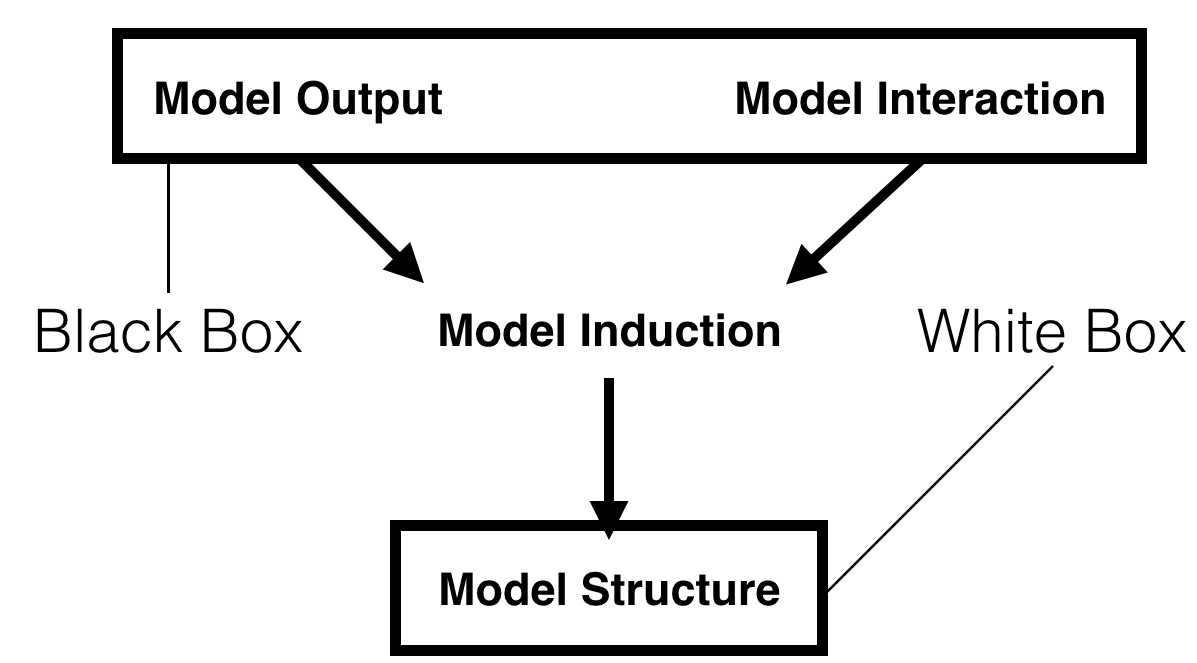
\includegraphics[height=11em]{figs/motivation/expl_classes}
\caption{
The relation of output-, interaction-, and structure-explanations.
With the help of model induction over a reduced or carefully selected
input, output- and interaction-explanations can utilize structure explanations
of simple machine learning models.
Output- and interaction-explanations can be created while treating the model
as black-box. This is not possible for structure explanations.
}
\label{figs:motivation_expl_classes}
\end{figure}

% The types of explanations can be broadly categorized into black box (output and interaction)
% and white box (structure) explanations as shown in \figref{figs:motivation_expl_classes}.
% Note that input explanations do not fall into either of those categories as they
% do not rely on any \emph{concrete} machine learning model due to focusing on data
% preparation and pre-processing.

% In this work we discuss exclusively input and black box explanations.
% Black box-, as opposed to white box-, explanations have the advantage that they can
% deal with any complexity of the underlying model.
% Developed techniques also do not need to be adapted to new algorithms emerging from
% machine learning research as long as the core interface (input produces prediction scores)
% remains the same.
% Furthermore, black box explanations also allow to compare the behavior of different
% algorithms which is otherwise not possible.
% Lastly, with good performing machine learning models being highly valued in certain
% domains stakeholders do not need to fully reveal their assets to analysts using
% black box explanations.

% \section{Overview}
% In the following we show how the previously mentioned different kinds of explanations
% can be utilized using tools we developed.

% At first we focus on tools that help with the data preparation step.
% SeekAView (see \chapref{sec:SeekAView}) helps detect unusual patterns in the data and
% provides a way to find associations between features using guided subspace analysis.
% With Patient-viz (see \chapref{sec:Patient-viz}) we show a tool to verify the integrity
% of patient records that are used to construct features for diagnosis prediction.
% The tool helped a group of machine learning modelers and practitioners refine their definitions for disease labels.
% COQUITO (see \chapref{sec:COQUITO}) is designed to ease cohort definition and construction in the medical context.

% \begin{figure}[b!]
\centering
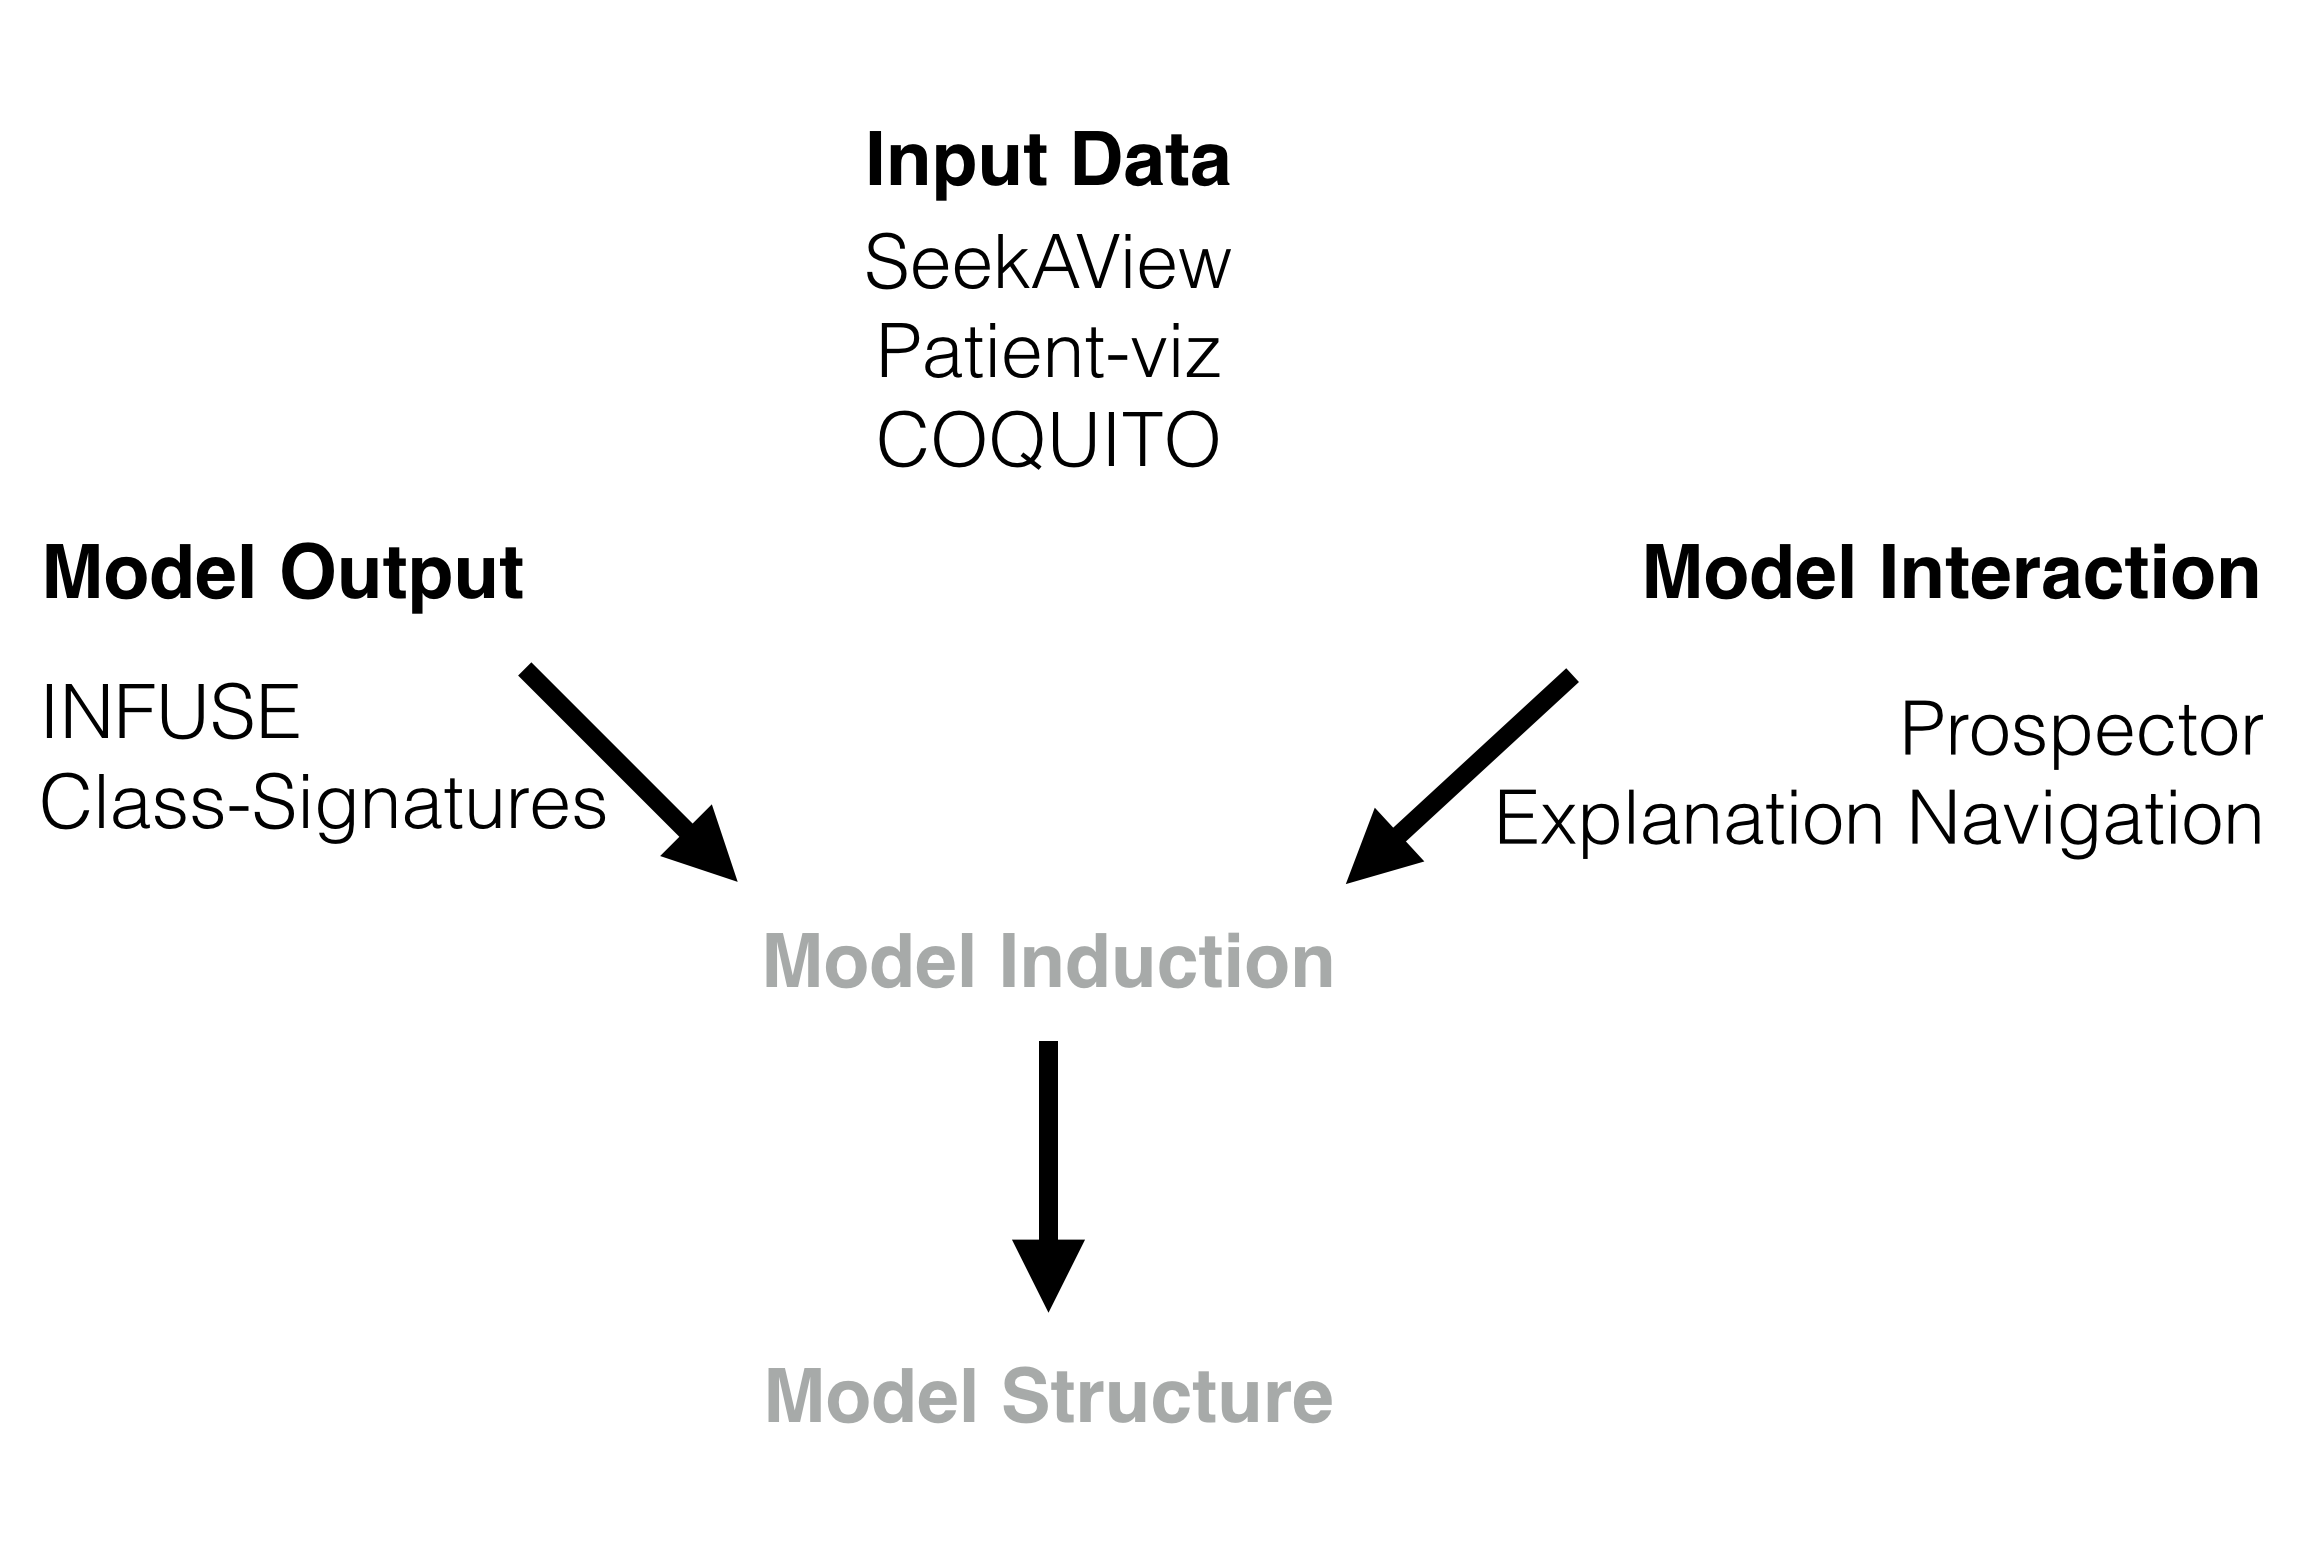
\includegraphics[height=14em]{figs/motivation/content}
\caption{
How the projects of my dissertation fit into the categorization of explanations
as shown in \figref{figs:motivation_expl_classes}.
As input data is focused on data pre-processing it doesn't appear in the
original figure. Furthermore, no works focusing on structure explanations are
presented as they require knowledge about the internal state of the model.
However, with \textbf{Class Signatures} model induction based on the original
model's outputs and subsequent structure explanations of the induced model are
part of the work-flow.
}
\label{figs:motivation_content}
\end{figure}

% Secondly, we focus on tools that use model interaction to explain model behavior.
% Those techniques search the output space of a model by manipulating the input space and differ mostly
% by their mechanism of probing the machine learning model.
% Prospector (see \chapref{sec:Prospector}) uses partial dependence to calculate the local
% influence of features.
% We are currently working on a tool that uses a different probing mechanism aimed at
% textual data which is described in \chapref{sec:Outlook}.

% Thirdly, we focus on tools using only the output of machine learning models to
% provide explanations.
% This category is especially useful if the model that produced the output cannot
% be shared or is otherwise not be available.
% The scope of model outputs can reach from feature rankings as shown with INFUSE (see \chapref{sec:INFUSE})
% to analyzing predictions scores (see \chapref{sec:Class-Signatures}).
% The latter is partially published ongoing work which we will revisit in \chapref{sec:Outlook}.

% In \chapref{sec:Outlook} we will describe current projects that fit in the categories described above.
% We further explore in which directions those projects develop and provide a time-line of their completion
% alongside a draft of final thesis' structure in \chapref{chap:outline}.
